\documentclass[a4,12pt]{article}

\usepackage[francais]{babel}
\usepackage[utf8]{inputenc}
\usepackage[T1]{fontenc}
\usepackage[babel=true]{csquotes}
\usepackage{amsmath}
\usepackage{amssymb}
\usepackage{float}
\usepackage{graphicx}
\usepackage{wrapfig}
\usepackage{hyperref}
\usepackage{array,multirow,makecell}
\usepackage[a4paper]{geometry}
\usepackage{eurosym}
\usepackage{xcolor}
\usepackage[
backend=biber,
style=alphabetic,
sorting=ynt
]{biblatex}

\geometry{hscale=0.80,vscale=0.80,centering}

\hypersetup{colorlinks = false,linkbordercolor = {white}}
\addbibresource{biblio.bib}
\frenchbsetup{StandardLists=true}
\usepackage{enumitem}
\setlength\parindent{20pt}
\begin{document}
\begin{titlepage}
\title{ E-Jam \\ Business Plan}
\author{Baumann Matthieu, Cornebize Tom, Jaskolski Aliocha, \\Fischman Adrien, Thiollière Guillaume.}
\end{titlepage}
\date{}

\maketitle

\rule[0.5ex]{\textwidth}{0.2mm}


\rule[0.5ex]{\textwidth}{0.2mm}

\newpage
\tableofcontents
\newpage

\section{Description du produit}


\subsection{Présentation générale}

E-Jam est un service web permettant à plusieurs musiciens de jouer ensemble en direct.
En connectant votre instrument à votre ordinateur, vous pourrez jouer à plusieurs,
chacun depuis chez soi grâce à internet.
Vous pourrez également écouter librement et en direct des personnes jouer.

E-Jam est composé de deux éléments. Un logiciel permettant aux musiciens de diffuser
la musique qu'ils jouent, et un site web permettant d'écouter une session, mais
également d'interragir avec les autres utilisateurs.

Nous présenterons dans un premier temps l'origine de cet idée et l'équipe qui
l'a concrétisée. Nous détaillerons ensuite le fonctionnement du logiciel et du
site web.



\subsection{Origine de l'idée}
L'idée d'E-Jam est directement venue de nos besoins respectifs. En effet, plusieurs
membres de l'équipe pratiquent un instrument et ont déjà œuvré au sein
d'un groupe de musique. Nous nous sommes rendu compte que le fait de constituer un
groupe et d'aménager des horaires compatibles avec les exigences de tout les membres du
groupe n'est pas une chose aisée.\\

Ces contraintes que sont par exemple l'heure de rendez-vous, le lieu de rendez-vous, la
location d'une salle de répétition, les problèmes de transports, les temps de préparation des
instruments (montage des cymbales sur une batterie, accordage des instruments, réglages du
volume de chaque instrument, réglages des pédales d'effets, etc.) nous ont poussé à nous poser
des questions sur les conditions d'amélioration des séances de répétition en groupe.
Conscient des avancées en matière de nouvelles technologies liées à l'informatique des
télécommunications, il est vite devenu évident pour nous d'exploiter le réseau internet afin
de pouvoir créer une plate-forme de répétition en ligne. Chaque membre d'un groupe
pourrait ainsi se connecter et répéter en live tout en restant chez soi, avec son matériel
et son confort de vie.

En outre, une telle application permet aux musiciens de réaliser de nombreuses
économies de temps et d'argent :

\begin{itemize}
\item le coût de la salle de répétition,
\item les coûts de transport (voiture, transports en commun),
\item les temps de transports,
\item le temps d'installation.
\end{itemize}

Le temps d'installation commun au groupe est largement minoré puisque chaque
musicien dispose du confort d'installation de son équipement chez lui. Ainsi, le
batteur n'a pas à régler la tension de ses peaux, installer ses propres cymbales
et modifier la disposition des toms.

Un tel gain en temps permettrait d'ailleurs au groupe de répéter plus longtemps. Prenons
un exemple concret où le temps de répétition d'un groupe de rock lambda est de deux heures
par semaine. Une estimation correcte et non exagérée reviendrait à affirmer qu'il faudrait
environ une dizaine de minutes à chaque début de séance de répétition afin de garantir que
tout les membres du groupe soit bien arrivés, installés et que le contrôle de volume de
chaque musicien soit effectué (appelée balance dans le jargon propre aux musiciens). Ainsi,
on estime à 8,33 \% le temps perdu de répétition pour ce groupe. Sur une année de répétition
que l'on peut estimer à 36 semaines sur 52, ce groupe perdrait alors 360 minutes de
répétition, c'est-à-dire pas moins de 6 heures de répétitions.\\

Là encore, notre application permettrait de passer outre une telle perte et même de
permettre à chaque groupe la possibilité de répéter 6 heures de plus sur une année.

\subsection{Présentation de l'équipe}

Notre équipe est constituée de cinq étudiants de l'Ensimag, passionnés d'informatique
et de musique.

\begin{itemize}
\item \underline{Guillaume Thiollière}
Responsable technique et développeur côté
serveur de l'application E-Jam. Guillaume est également initiateur
d'une étude financière poussée permettant la quantification de nos
coûts et de nos revenus. Il pratique également la guitare classique
depuis de nombreuses années.

\item \underline{Tom Cornebize}
Responsable technique et développeur côté client
de l'application. Initiateur de l'étude de marché quantitative de notre
produit : mise en place d'un sondage permettant d'évaluer un marché
pour notre produit.

\item \underline{Matthieu Baumann}
Responsable technique et développeur du site
web E-Jam. Initiateur d'une étude de marché plus qualitative basée sur la
discussion avec des acteurs du monde de la musique. Il pratique
également de la guitare électrique et a déjà œuvré en tant que musicien
dans plusieurs groupes.

\item \underline{Adrien Fischman}
Responsable technico-commercial et juridique.
Adrien s'occupe de la partie législative relative à notre projet ainsi que
de plusieurs aspects financiers tels que l'étude de rentabilité de notre
produit de par ses moyens de revenus inhérents. Il est également
musicien.

\item \underline{Aliocha Jaskolski}
Responsable technico-commercial. Initiateur d'une
étude de la concurrence poussée permettant à E-Jam d'adapter sa stratégie
à la situation actuelle et ainsi, de se renseigner sur les moyens de se faire
valoir tant populairement que financièrement. Responsable publicité. Il
pratique la guitare électrique.

\end{itemize}

Le besoin dont E-Jam répond a été exprimé de par une constatation et réflexion de
l'ensemble des membres de l'équipe. C'est pourquoi, tous sont à l'origine du produit E-Jam.


\subsection{Logiciel}

Nous présentons ci après les fonctionnalités de base de E-Jam.

Lors du premier lancement du logiciel il est nécessaire de créer un compte. Ce compte permettra d’identifier les utilisateurs et offrira des fonctionnalités telles que suivre un musicien et être alerté lorsqu’il se connecte ainsi que gérer ses évènements.
Une fois le compte créer le musicien peut rechercher une session ou créer une session. Il a aussi accès à son agenda.
\begin{itemize}
    \item \textbf{Créer une session} \\
    Pour créer une session l'utilisateur doit remplir différents champs qui caractériseront la session. Ces champs sont :
    \begin{itemize}
        \item \textbf{le nom :} un mot
        \item \textbf{la description :} une phrase
        \item \textbf{le style de musique :} un ensemble de mot-clé parmi ceux proposés
        \item \textbf{le niveau des musiciens :} un mot-clé parmi ceux proposés
        \item \textbf{les instruments autorisés :} un ensemble de mot-clé parmi ceux proposés
        \item \textbf{type de session :} public ou privé
        \item \textbf{latence maximale tolérée } (l'intérêt de ce champ sera précisé dans la partie technique)
        \item \textbf{etc.}
    \end{itemize}
    \item \textbf{Rejoindre une session}\\
    Pour rejoindre une session l’utilisateur écrit l’instrument qu’il joue, son niveau, le style souhaité, sa localisation. Le logiciel propose alors un ensemble de résultat correspondant à sa requête.
    \item \textbf{Accéder à son agenda}\\
    E-Jam propose aussi un système d’événements renforçant les interractions entre utilisateurs. Un événement indique la création d’une session à une date donnée ainsi que les caractéristiques de cette session. Un musicien peut alors créer un événement ou marquer sa participation. L’utilisateur peut consulter son agenda avec la liste des évènements auxquels il participe, des évènements proposé par ses amis ainsi que des évènements qui peuvent l'intéresser.\\
    Le but de ce mécanisme et de permettre au musicien de se rejoindre facilement à des dates établies ainsi que de faire découvrir certaine session de jeux en proposant des évènements en dehors de son cercle d’ami. Les évènements proposé seront en fonction des goût de l’utilisateur mais aussi en fonction de se localisation pour permettre aux musiciens proche de se découvrir.\\
    \\
    Une fois que le musicien est dans un session il peut jouer de la musique et entendre les autres membres de la session. Il a aussi accès à des outils pour facilité l’organisation de la session:
    \begin{itemize}
        \item accordeur
        \item tchat et vidéo-conférence
        \item métronome
        \item playback
        \item partitions
        \item etc.
    \end{itemize}
\end{itemize}

\subsection{Plate-forme en ligne}
E-Jam propose aussi une plate-forme en ligne pour les spectateurs. La création d'un compte est possible pour les spectateurs, mais non nécessaire. L’utilisateur se verra proposé des sessions sur la page principale et pourra aussi rechercher une session avec des mots-clés et des noms de musiciens ou groupes.\\
La création de compte permettra aux spectateurs d’avoir un agenda avec les dates des sessions des musiciens qu’ils suivent.

Nous avons développé un prototype de plate-forme en ligne.

La figure \ref{ceca_site_accueil} est une capture d'écran de la page d'accueil de
la plate-forme. On y voit notamment différentes sessions, chacune étant dotée d'un
ou plusieurs tags qualifiant son style de musique ainsi que de compteurs du nombre
de musiciens et du nombre de spectateurs. L'utilisateur a également accès à une
barre de recherche lui permettant de chercher une session ou un utilisateur selon
différents critères. Il y a également un menu latéral, donnant accès au profil de
l'utilisateur, sa messagerie, son agenda, ses favoris (i.e. les autres utilisateurs
qu'il apprécie) ainsi qu'un bouton permettant de démarrer une nouvelle session.

\begin{figure}[!ht]
    \center
    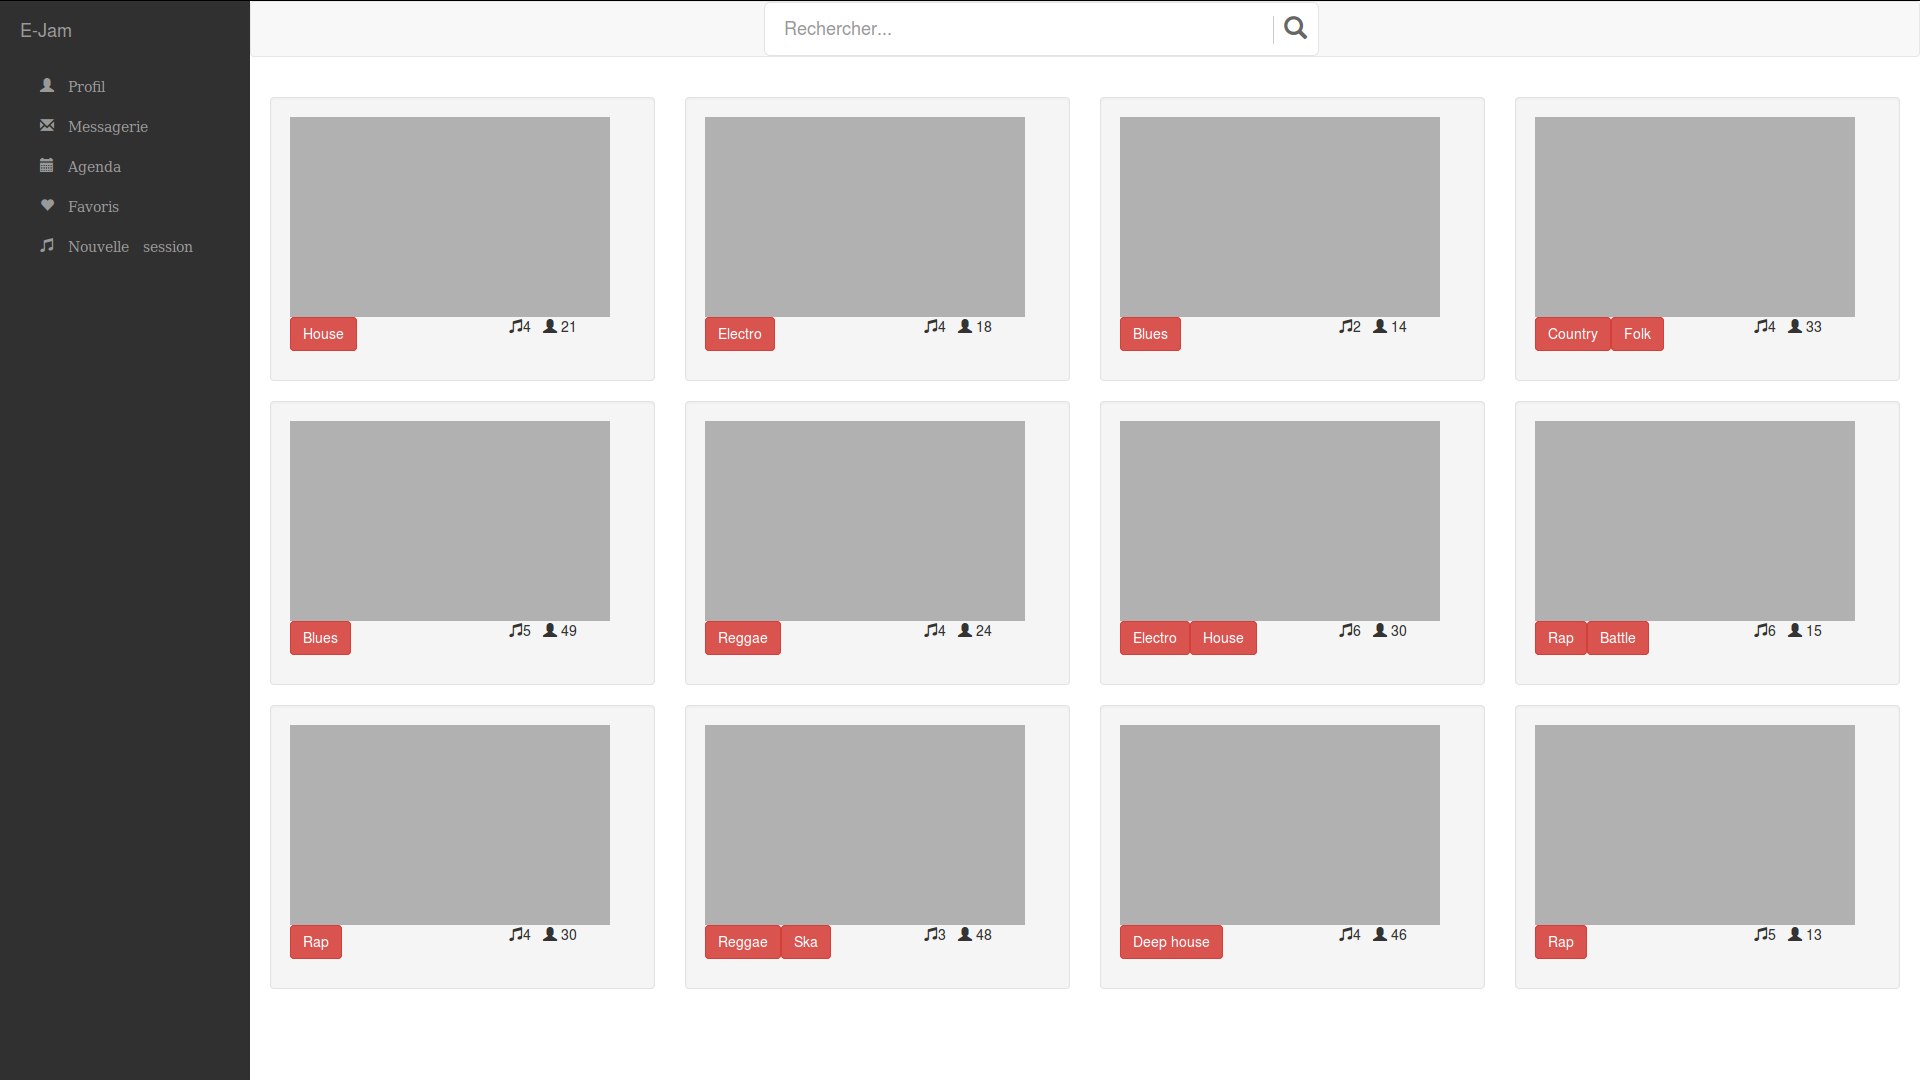
\includegraphics[width=15cm]{ceca_site_accueil.png}
    \caption{Page d'accueil de la plate-forme en ligne}
    \label{ceca_site_accueil}
\end{figure}

La figure \ref{ceca_site_session} est une capture d'écran d'une session. Cette page
présente, comme la page d'accueil, une barre de recherche et un menu latéral.
La partie spécifique à la session est divisée en deux.

La partie gauche est dédiée aux actions de l'utilisateur. Une barre d'onglets permet
d'alterner entre les différentes utilisations :
\begin{itemize}
    \item L'utilisateur peut discutter avec d'autres utilisateurs (spectateurs ou
    musiciens).
    \item L'utilisateur peut modifier les paramètres de la session, il a notamment
    accès à un equalizer.
\end{itemize}

La partie droite est dédiée à la visualisation, qui peut être modifiée par les musiciens :
\begin{itemize}
    \item Les musiciens peuvent se filmer en train de jouer et diffuser la vidéo ici.
    \item Ils peuvent diffuser une vidéo pré-enregistrée ou une image fixe.
    \item Ils peuvent également diffuser des effets visuels.
\end{itemize}

\begin{figure}[!ht]
    \center
    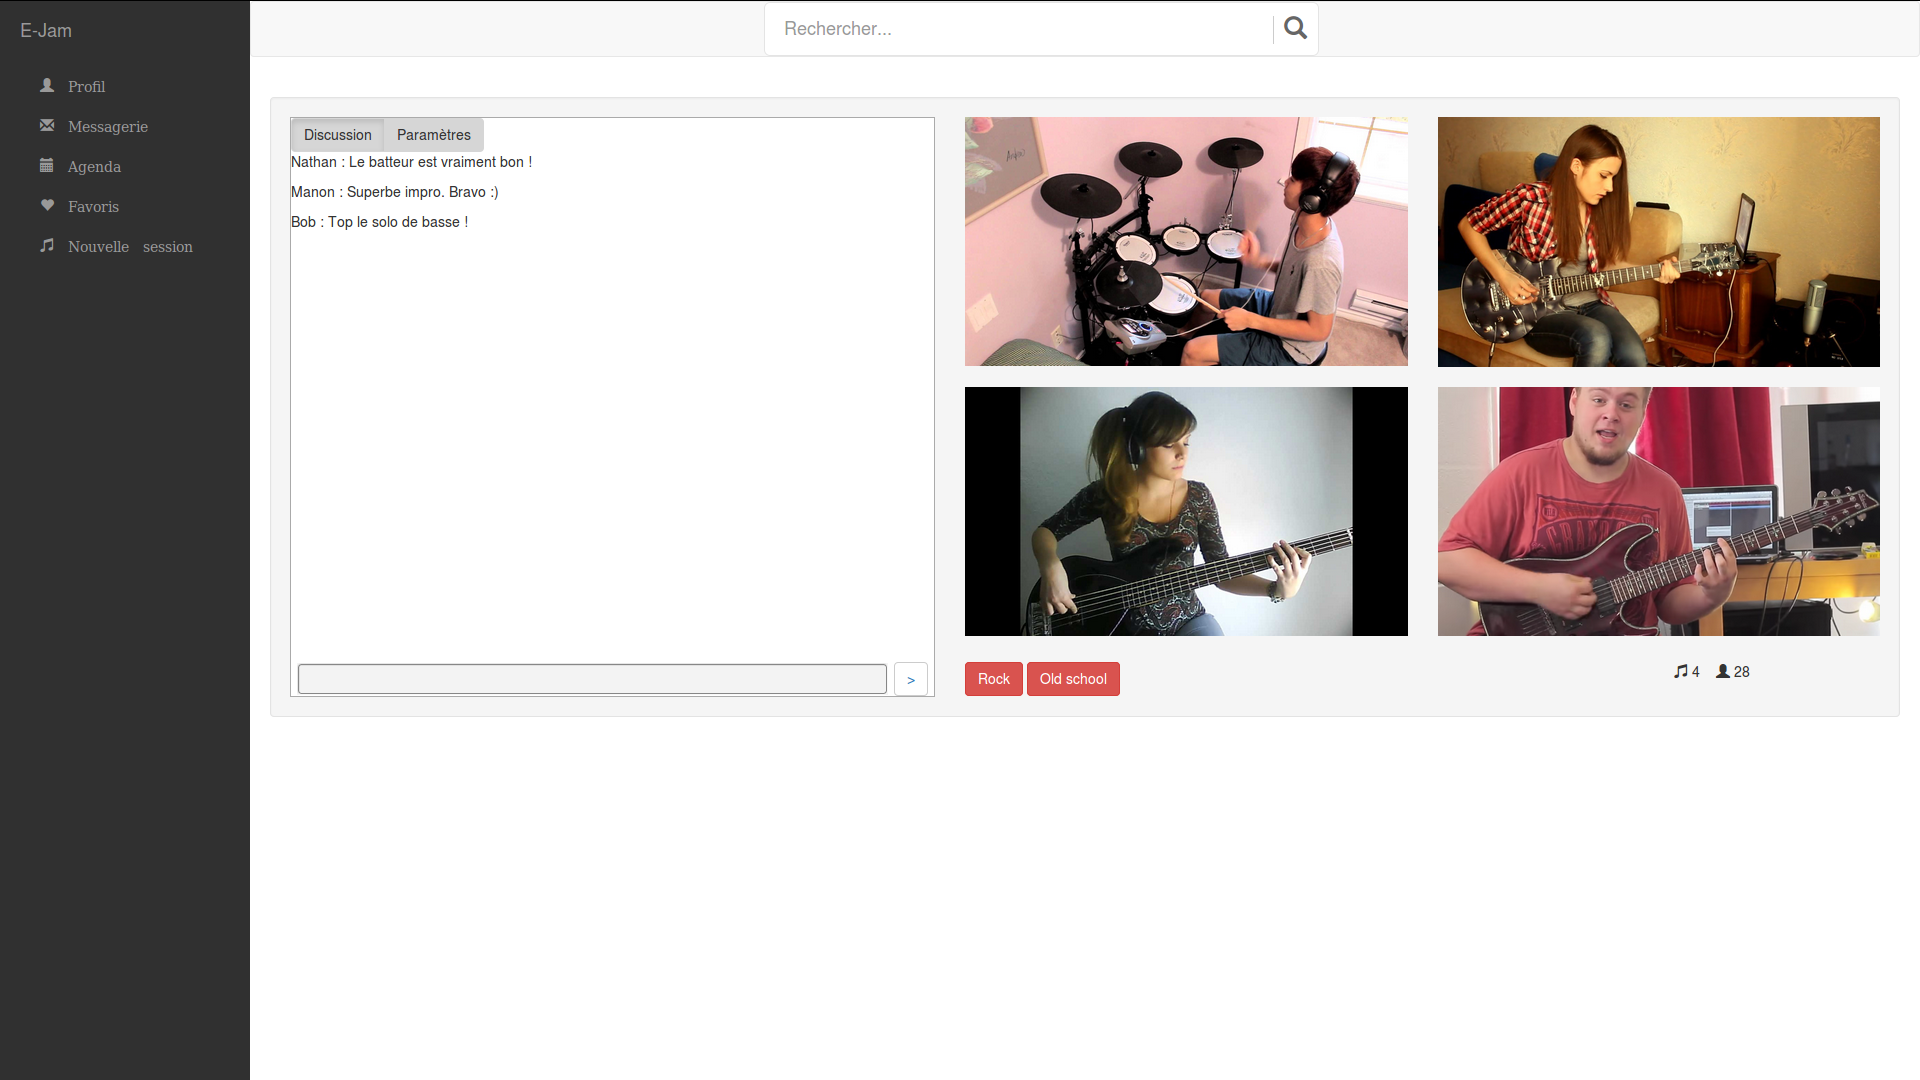
\includegraphics[width=15cm]{ceca_site_session.png}
    \caption{Une session sur la plate-forme en ligne}
    \label{ceca_site_session}
\end{figure}

\subsection{Offre Premium}

Un utilisateurs de Ejam peut souscrire à un abonnement premium de 5 euros par mois. Cet abonnement lui donnera
accès à plus de fonctionnalités et de confort d'utilisation :

\begin{itemize}
    \item \textbf{Gestion du public}\\
		L'utilisateur premium pourra poster ses sessions sur le calendrier public. Le nombre de spectateur par session ne sera pas limité.
    \item \textbf{Sessions plus complètes}\\
		Un ensemble de partitions, de playback et d'effets sonores sera mis à disposition des musiciens disposant d'un compte premium.
    \item \textbf{Enregistrement des sessions}\\
        Les musiciens disposant d'un comtpe premium pourront enregistrer les sessions auxquelles ils participent, leur permettant de les garder en diffusion libre ensuite.
    \item \textbf{Sessions privées}\\
        Le compte premium offre également la possibilité d'organiser des sessions privées, permettant un contrôle total des droits d'accès pour les autres musiciens ainsi que le public.
    \item \textbf{Pas de publicités}\\
        Aucune publicités ne seront affichés pour les utilisateurs disposant d'un compte premium.
\end{itemize}

Les comptes premiums, ouverts à tous les utilisateurs, ciblent ainsi d'avantage les musiciens que les utilisateurs n'étant que spectateurs.

\subsection{Détails sur la réalisation technique}

Dans une session chacun des musiciens envoi aux autres ce qu’il joue. Or cette transmission de donnés peut être plus ou moins longue selon la distance entre les utilisateurs et l’état du réseaux. Ce qui pose le problème suivant: le temps de transmission est-il perceptible par le destinataire ? Car si un guitariste reçoit le tempo du batteur une demi seconde en retard lorsqu’il joue sa note le batteur la percevra décalé avec ce qu’il joue même si le guitariste joue sur le tempo.\\
Le problème que l’on cherche à résoudre est quelle est la latence limite avant que les musiciens ne soient gêné.\\
Selon un ingénieur du son, le temps de délais maximal imperceptible est de l’ordre de 30ms. Aussi nous avons fait différents tests:
\begin{itemize}
    \item \textbf{Précision des musiciens}\\
    Pour savoir à quelle précision on savait jouer en rythme : on essayait de jouer sur le tempo et on calculait la différence réelle entre le tempo et ce que l’on jouait. La précision était de l’ordre de quelques dizaines de milli-seconde.\\
    Cette expérience nous confirme que la précision des musiciens n’est pas en deçà de la dizaine de milli-seconde.
    \item \textbf{Temps minimal pour percevoir deux sons différents en condition réelle}\\
    Pour savoir à partir de quel délai on pouvait percevoir la différence entre deux son en condition réelle : on jouait une note sur un ordinateur, qui était automatiquement rejouée après un délais de durée paramétrable.
    \\
    On a observé que pour 30ms on ne percevait qu’un seul son et la différence ne pouvait s’entendre qu’à partir de 60ms.
\end{itemize}
\newpage
\section{Stratégie}
\subsection{Analyse qualitative de l'étude de marché}
Nous nous sommes entretenu avec plusieurs contacts venant de milieux professionnels variés afin d'en savoir plus sur l'existence d'un marché qui nous serait profitable. De façon globale, l'ensemble de nos contacts, à savoir plusieurs gérants de magasins de musique, un ingénieur du son ainsi que des connaissances personnelles ont été conquis par l'idée. Ainsi, nombreux sont ceux qui sont intéressés par une telle plateforme Web interactive leur permettant de jouer avec leur amis et en temps réel.\\
\\

\textbf{Guitar Land Grenoble :}
    Notre premier contact fut le gérant du magasin de musique Guitar Land de Grenoble. L'idée lui semblait très pertinente. Il a d'ailleurs exprimé le fait qu'un jour il puisse essayer l'application si une telle plate-forme sortirait à l'avenir. En revanche, il n'en exprime pas directement le besoin car ce dernier possède déjà un groupe actif et une salle de répétition leur permettant de se produire une fois par semaine. Il semblait quelquefois un peu dubitatif sur l'aspect réalisabilité technique du projet, plus particulièrement concernant les problèmes de latence auxquels devront faire face l'application et le serveur afin de maintenir une connexion satisfaisante pour les musiciens.\\
    \\
    Notre discussion a abouti sur de nombreuses idées d'ajout de fonctionnalités au sein des sessions permettant la répétition de plusieurs musiciens ensemble. Parmi celles-ci on retrouve :
    \begin{itemize}
        \item L'ajout d'un accordeur en ligne simple et intuitif permettant aux musiciens de définir un accordage commun et en relation avec le style de musique joué durant la session de répétition. Par exemple, des accordages spéciaux pour le blues, le jazz ou le classique.
        \item La possibilité d'intégrer par défaut des outils rythmiques tels qu'un métronome permettant à chacun de suivre un tempo donné. Plus généralement, des rythmes prédéfinis, connus et communs à des styles bien particuliers pourront enrichir l'expérience musicale et livrer une réelle immersion notamment pour l'improvisation et l'apprentissage. Ainsi, si les musiciens d'une session manquent d'un instrument, il leur est possible d'ajouter d'autres mélodies et instruments à partir d'une interface intuitive des sessions d'E-Jam.
        \item Enfin, notre contact a déclaré qu'il serait souhaitable d'intégrer un module vidéo permettant aux musiciens de dialoguer entre eux (avant le début d'une session par exemple) et ainsi se mettre d'accord sur la suite de notes, de rythme, de tonalité avec lesquelles ils répéteront. Cette fonctionnalité, très utile permettrait aux musiciens d'apprécier pleinement les répétitions en fixant un certain cadre pour tous et ainsi d'éviter toute frustration du à des problèmes de compréhension par exemple.
    \end{itemize}
Notre contact a également déclaré qu'il donnait quelques cours de musiques. Nous lui avons présenté E-Jam comme une plate-forme en ligne lui permettant de donner des cours en ligne de chez lui. L'idée lui semblait bonne et selon lui, pourrait découler sur une autre facette d'E-Jam. Il a toutefois déclaré qu'il n'utiliserait pas l'application dans ce sens puisque personnellement, il lui est important de corriger ses élèves jusque dans leur gestes (position des doigts sur un manche de guitare, posture générale, etc.). À l'inverse, nous avons consulté de nombreuses personnes disant qu'elles révéraient d'obtenir des cours en ligne de musiciens célèbres et n'hésiteraient nullement à payer ces cours plus cher.\\
\\

\textbf{Bertet Musique :}\\
Nous avons aussi discuter avec une employée de Bertet Musique. Comme le premier contact elle était intéressée pour tester le projet et se questionnait un peu sur les difficultés techniques mais n’avait pas d’a priori sur le sujet.\\
Elle a évoqué le fait que les sessions devaient permettre de s’organiser facilement avec notamment un tchat, la gamme utilisée, la grille d’accord, l’ordre des improvisations, leurs durées, etc.\\
Le logiciel lui semblait utile pour pouvoir répéter avec des amis sans toujours se déplacer mais aussi de pouvoir jouer beaucoup plus facilement avec d'autres musiciens.
Aussi le logiciel pouvait être utile pour faire découvrir des musiciens pas loin de chez soi et pour créer des liens entre musiciens.\\

Finalement cet entretiens nous a permis de réfléchir à de nouvelle fonctionnalité pour l’interface utilisateurs des sessions, ainsi que d’aborder plus en profondeur les fonctionnalité sociale qu’on pourrait proposer.

\subsection{Analyse quantitative, étude de marché, questionnaire}
Nous présentons ici une synthèse des résultats du questionnaire que nous avons diffusé. Cette synthèse est sujette à évolution, trop peu de personnes ayant répondu (44 personnes) et l’échantillon étant peu représentatif (81\% des personnes ayant répondu ont entre 18 et 25 ans). Nous avons prévu d’élargir le cercle de diffusion.\\
\\
Nous notons que 50\% des répondants sont musiciens. Parmi ces musiciens, 86\% sont intéressés par jouer avec des amis, 64\% avec des professeurs, 54\% avec des inconnus et 50\% avec des artistes renommés.\\
Le faible nombre de personnes voulant jouer avec des inconnus ou des artistes renommés nous a surpris.\\
\\
Parmi l’intégralité des répondants, 82\% sont intéressés par écouter des artistes renommés, 75\% des amis, et 57\% des inconnus. Cela confirme la première observation que les répondants semblent moins intéressés par de la musique jouée par des inconnus que par leurs amis. De plus, ils semblent plus intéressés par écouter des artistes renommés que par jouer avec eux.\\
\\
Ces deux observations soulèvent des questions importantes quant aux fonctionnalités que nous devons proposer. Ainsi, il semble très important de permettre la création de relations entre les utilisateurs, à la manière des “amis” sur Facebook ou des “followers” sur Twitter. Il faut également organiser la diffusion de lives d’artistes renommés.
Il semble moins important de permettre d’écouter ou de jouer avec des inconnus. Ainsi, il ne serait pas forcément utile d’apporter à nos utilisateurs des suggestions de personnes à écouter ou avec qui jouer, selon leurs goûts et leurs capacités (dans le cas des musiciens).\\
Toutefois, ces résultats sont à relativiser. On peut faire le parallèle entre ce que nous proposons, soit jouer à distance et en direct de la musique, et les jeux vidéos en ligne, soit jouer à distance et en direct à un jeu vidéo. Il y a quelques années, peu de monde aurait été séduit par l’idée de jouer à un jeu avec des inconnus. C’est pourtant ainsi que fonctionnent la plupart des jeux en ligne aujourd’hui.\\
\\
Notre questionnaire révèle que parmi les répondants, 27\% seraient prêt à payer un abonnement, et 30\% seraient prêt à participer à une campagne de financement. Ces nombres sont très satisfaisants même si la réalité est certainement de deça.\\
%changement car dans le dimensionnement je dis que le modèle premium est bon si il y a 5-10% de premium (chiffre obtenu de blog etc...)
\\
Finalement, les répondants ont globalement un temps de latence satisfaisant, mais de grandes disparités existent. Le temps de latence médian est de 30ms, le minimum est de 2ms et le maximum est de 105ms.
Il serait donc impossible pour certains des répondants d’utiliser notre outil pour jouer de la musique. L’écoute restera possible, puisqu’un plus grand temps de latence n’est pas gênant.
Le jeu en direct devrait être possible pour la moitié des répondants, si l’on fixe la latence limite à 30ms.
\subsection{Analyse de la concurrence}
Nous nous sommes intéressés à l’offre déjà disponible sur internet, proposant des sessions live de musique. Même si l’offre est peu développée, une poignée de sites proposant des services similaires existent déjà.\\
Il nous est apparu que le logiciel libre Ninjam, était notre concurrent le plus sérieux tant par son nombre d’utilisateurs (notamment en France) que par sa fiabilité. Des sites comme ninbot.com, utilisant ce logiciel libre, peuvent enregistrer jusqu’à 100 musiciens en simultanée, et le forum est très actif. Les lives proposés sont d’une très bonne qualité acoustique. Cependant leur approche du problème de la latence est différente de la notre : une mesure de retard est imposé à tous les musiciens voulant jouer ensemble, ce qui permet d’ajuster les musiciens entre eux. L’expérience est différente de la manière de jouer de la musique traditionnellement, mais à en croire la plupart des utilisateurs cela reste ludique. L’interface du logiciel, quant à elle, semble compliquée et s’adresse à des musiciens motivés, maîtrisant les bases en solfège et en informatique.\\
D’autres sites comme jammr ou sofasession par exemple, proposent également de jouer en simultanée, mais souffrent d’une communauté réduite (moins de 1000 likes sur facebook), ou d’un site en beta et donc non-fonctionnel pour l’instant. Le problème de la latence est souvent résolu par la méthode de ninjam (une mesure de retard). Nous avons noté que Sofasession dispose d’une interface très facile et agréable d’utilisation, et d’un aspect réseau social bien pensé.
Mis à part Sofasession, qui ne semble pas avoir de sources de revenus, tous ces sites ont en commun de proposer (ou de vouloir proposer à l’avenir après la phase de beta) un compte premium, permettant l'accès à de nouveaux services, ou un accès moins limité aux services de base. Il peut s’agir par exemple de jams privés, enregistrement individuels ou de mixer en ligne.\\
\\
En conclusion : mis à part ninjam qui jouit d’une communauté active, l’offre parait peu développée pour l’instant, et celle qui existe utilise le procédé de la “mesure de retard” pour traiter le problème de la latence.

\subsection{Positionnement par rapport à la concurrence}
Nous allons nous intéresser ici à notre stratégie notamment par rapport à la concurrence vue précédemment.\\
\\
Notre projet profite des avancés technologique en matière de réseaux: amélioration des débits, diminution du temps de latence et robustesse de la connexion. Cela permet de nous différencier des concurrents qui ont choisi de faire jouer les musiciens avec un délai (une mesure pour Ninjam), technique utilisée afin de palier les problèmes de latence que posait le réseau internet mondial de l’époque.\\
Aussi bien que nous soyons aussi limité par la latence puisqu’on ne pourra pas jouer ensemble entre Paris et Tokyo, on pourra profiter des améliorations futures des temps de latence (bien qu'il soit borné par la vitesse de la lumière).\\
\\
D'autre part, nous avons décidé avec E-Jam, de mettre l'accent sur une gestion des sessions simple, intuitive et la recherche de session de jeu. On veut rendre l'expérience utilisateur la plus agréable possible et c’est aussi un point crucial pour créer et entretenir une communauté autour de notre projet. Nous voulons placer la créativité musicale au centre de tout c’est pourquoi nous avons opté pour une interface des plus simple et rapide permettant à l’utilisateur musicien de rejoindre des sessions selon ses propres critères à savoir :
\begin{itemize}
    \item les sessions occupées par ses amis,
    \item les sessions en accord avec son style de musique (rock, jazz, improvisation, etc.),
    \item les sessions correspondant à son niveau de jeu.
\end{itemize}
Enfin toujours pour développer la communauté nous ajouterons au logiciel l'interface pour les spectateurs, nous organiserons des évènements avec des artistes renommés et nous permettrons à des groupes de se faire connaître notamment avec l’aide de tremplins.\\
\\
Nous n’ avons pas d'innovation technologique réelle, par conséquent une concurrence directe pourrait apparaître (en plus de Sofasession qui est un projet assez proche) et proposer des services très proches des nôtres.\\
Enfin pour toutes les fonctionnalités annexes comme le fait de pouvoir assister à une session en tant que spectateur ou de participer à un tremplin, il existe une concurrence indirecte : les festivals, ainsi que les sites comme Soundcloud ou Youtube qui permettent d'écouter de la musique fait par des musiciens plus ou moins amateurs.

\section{Dimensionnement et financement}

Le projet commencera par une phase de développement réalisée par nous même. Cette
étape durera six mois et a pour but la création du site web ainsi que du logiciel.
Nous ne nous verserons pas de salaire durant cette phase.

E-Jam sera officiellement lancé en janvier 2017.

Selon une enquête du DEPS faite en 2008 [Figure ~\ref{fig:pratiques}]
12\% des français de plus de 15 ans pratiques d'un instruments de musique et 23\% savent
jouer d'un instrument de musique.
Avec les études de marché précédentes, nous pensons pouvoir prendre un marché potentiel de 10\% de la population française.\\

\begin{figure}[!h]
    \centering
    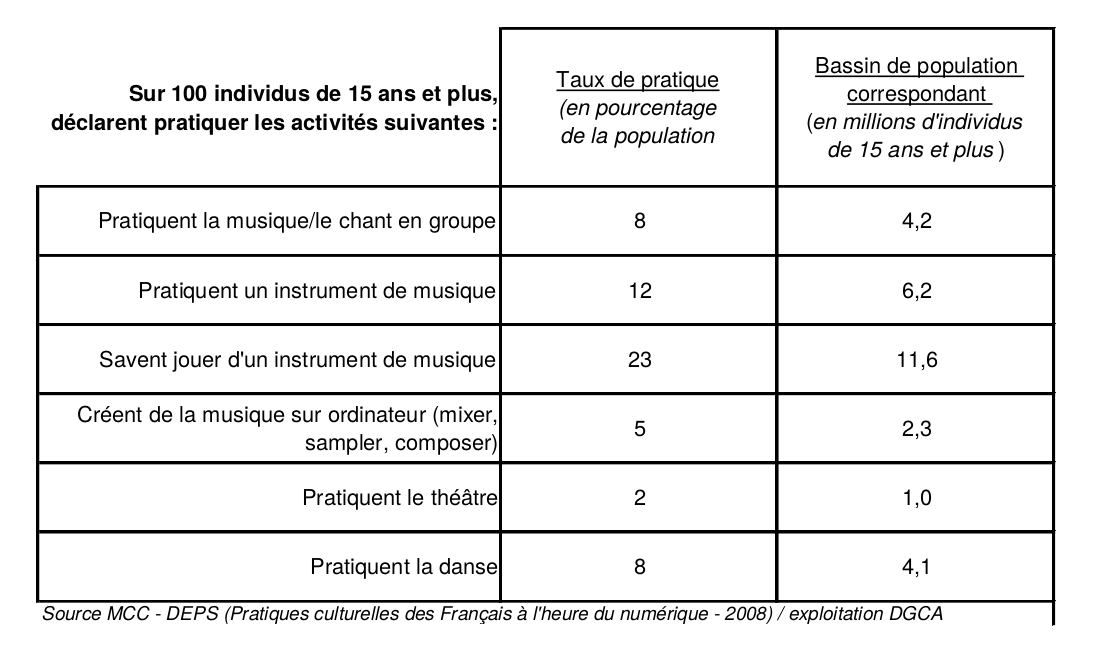
\includegraphics[width=400pt]{pratiques_culturelles_des_francais.png}
    \caption{pratiques culturelles des français}
    \label{fig:pratiques}
\end{figure}

Nous espérons séduire 1\% de ce marché potentiel d'ici 2020, soit environ 60000
utilisateurs.
Ce nombre peut être atteint en multipliant par 1.6 le nombre d'utilisateurs tous
les ans, en partant de 12000 utilisateurs dès la première année.
Pour cela, nous misons sur une très forte présence sur les réseaux sociaux.

\subsection{Moyens matériels}

%exemple de openmailbox.org
Domains name: 120\euro\\
Ssl certificate : 144\euro\\
Infrastructure : 13720\euro\\

\subsection{Moyens humains}

Nous distinguons deux types de postes différents nécessaires à E-Jam.

\begin{itemize}
    \item \textbf{Trois informaticien(e)s}\\
    Ces personnes auront des tâches diverses liées à la maintenance et l'amélioration d'E-Jam.
    On peut notamment citer la correction de bugs, le développement de nouvelles
    fonctionnalités et la gestion des serveurs.
    \item \textbf{Un(e) responsable de la communication}\\
    Cette personne aura la charge de promouvoir E-Jam. Ceci inclut une forte présence
    sur les réseaux sociaux (aussi connu sous le nom de community manager), mais
    également la gestion de nos campagnes de publicité.
\end{itemize}

Nous prévoyons une rémunération de 2200\euro\ brut par mois et par salarié.

\subsection{Revenus premium}

E-Jam proposera à ses utilisateurs un compte premium offrant plus de fonctionnalités,
à un prix fixé à 5 euros par mois.

Le nombre d'abonné premium est en général aux alentours de 5\%. En effet les grands acteurs qui utilisent un modèle premium comme Skype ont un taux un peu inférieur à 10\%, d'autre part les site comme webmarketing-com conseille un taux vers 5\%. Un taux infèrieur ferait surfacturer la version premium et un taux trop supérieur serait dû à une version gratuite pas assez attractive pour les autres utilisateurs.\\

En prenant pour objectif 60 000 utilisateurs en 2020, nous pensons avoir 3 000 utilisateurs avec un compte premium à cette date.

\subsection{Revenus publicitaire}

Le site web ainsi que le logiciel afficheront de la publicités aux utilisateurs
ne disposant pas de comptes premium.

Selon eMarketer [Figure ~\ref{fig:revenu_par_utilisateur}] le revenu publicitaire par utilisateur de réseaux sociaux comme twitter et facebook est en hausse. Au cours des dernières années le revenu par utilisateurs par an pour ces réseaux est de l'ordre de 10 dollars.\\

On estime alors que le revenu que l'on pourra générer par utilisateur sera de l'ordre de 5 euros par an.

\begin{figure}[!h]
    \centering
    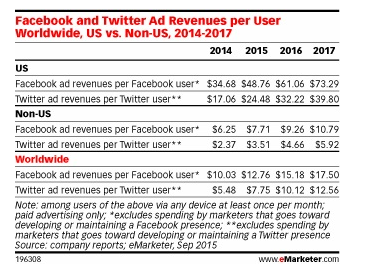
\includegraphics[width=300pt]{revenu_par_utilisateur.png}
    \caption{revenu par utilisateur}
    \label{fig:revenu_par_utilisateur}
\end{figure}

\subsection{TODO tableaux excels}

Calculs de coûts (chaine de valeur), seuil de rentabilité, compte de résultats prévisionnel, tableau de trésorerie et plan de financement.\\

\section{Aspect juridique}
Une plate-forme tel qu'E-Jam soulève différents problèmes. Notamment, en ce qui concerne le droit de représentation d'une oeuvre lors de reprises, de musiques déjà existantes, faites par des utilisateurs, mais aussi sur la notion d'oeuvre de collaboration et enfin sur la responsabilité d'E-Jam.

\subsection{Droit de représentation d'une oeuvre}

Un utilisateur qui n'est pas autorisé par l'auteur à faire une reprise de son oeuvre viole son droit de représentation qui est "la communication de l'oeuvre au public par un procédé quelconque".\\
Dès lors, il faut demander l'autorisation préalable de l'auteur ou de la SACEM (Société des Auteurs Compositeurs et Editeurs de Musique) à qui l'auteur aurait cédé les droits de représentation.\\
Pour éviter que ce soit à l'utilisateur de demander systématiquement l'autorisation, il est préférable que E-Jam conclut un contrat avec la SACEM afin que les auteurs perçoivent une rémunération à chaque fois qu'un de leur titre est repris.\\
\\
Cependant, contrairement à une boite de nuit, E-Jam ne peut pas prédire à l'avance le contenu de la plate-forme. Ainsi, même avec un contrat avec la SACEM, E-Jam aura l'obligation de vérifiaction des contenus illicites présents sur la plate-forme.\\
\\
Toutefois, les exceptions au droit d'auteur sont fixées à l'article 122-5 du code de la propriété intellectuelle et y figure "la représentation dans le cercle de famille" qui correspond à un cercle très restreint. La représentation privée doit être gratuite et effectuée exclusivement dans un cercle de famille : parents ou familiers. Donc si une oeuvre est uniquement publié entre les musiciens eux-mêmes, il n'y a pas besoin de rémunérer les artistes et de faire appel à la SACEM. Ce sera notamment le cas des sessions privées auxquelles donneront accès les comptes premium.

\subsection{Oeuvre de collaboration}

La qualité d’auteur appartient à celui sous le nom duquel l’oeuvre est divulguée.\\
Donc si un particulier met en ligne (donc divulgue) sa propre musique à son nom sur la plateforme, elle sera sa propriété. D’autre part, si un utilisateur créée une musique avec d’autres utilisateurs via la plateforme, l’oeuvre sera qualifiée d’ « oeuvre de collaboration » et elle sera la propriété commune des co-auteurs.

\subsection{Responsabilité de E-Jam}

Il faut différencier les qualités d'éditeurs et hébergeurs de musique.\\
Un éditeur de musique se différencie car il met à disposition du public son contenu qui devient modifiable. Dans ce cas, la mise à disposition des contenus musicaux relève de la responsabilité civile et pénale de E-Jam.\\
Un hébergeur (comme Youtube) n'est pas résponsable des contenus illicites. Il n'est pas soumis à une obligation générale de surveillance. Sa responsabilité n'est pas engagée, s'ils n'ont pas eu connaissance effective de la présence du contenu illicite. Il est responsable uniquement s'il n'agit pas pour retirer le contenu litigieux. Il n'a pas à retirer le contenu illicite sans notification préalable et même si ce contenu a déjà fait l'objet d'un signalement et a déjà été retiré une première fois.\\
Cependant, on ne peut pas réellement prédire à l'avance la qualification juridique de E-Jam. C'est le rôle actif ou non de la plateforme sur les contenus qui permet de retenir la qualité d'hébergeur et son régime de responsabilité. Cependant, c'est à la jurisprudence de déterminer. Toutefois, un accord avec la SACEM devrait résoudre ces difficultés.\\
\\
En ce qui concerne le rôle d'E-Jam dans les oeuvres de collaborations. Il faut prévoir un contrat avec les utilisateurs afin de déterminer l'influence qu'à E-Jam sur la création musicale. Bien qu'en aucun cas le droit de modifier ou dénatuer une oeuvre sans le consentement de l'auteur n'est possible, l'existence du contenu sur la plate-forme E-Jam et son maintient ou non, par E-Jam, sur la plate-forme proposé nécessite un contrat passé avec les utilisateurs pour délimiter les droits d'E-Jam.


\section{Conclusion}

E-Jam a pour but d'utiliser les grandes avancées technologiques faites dans les
domaines de l'informatique et des télécomunications pour apporter du confort et de
nouvelles opportunités aux musiciens. Répéter sans sortir de chez soi, mais aussi
trouver un public et faire des rencontres inattendues, telles sont les possibilités
offertes par E-Jam.

En suivant ce plan d'action, porté par une équipe d'étudiants passionnés par la
musique et l'informatique, E-Jam réalisera ses objectifs financiers et atteindra
les 60 000 utilisateurs pour un bénéfice net de 232000\euro\ d'ici l'année 2020.

Pour cela, un investissement de 15000\euro\ est nécessaire afin de réaliser la première année.
Saisissez cette opportunité et investissez dans E-Jam, une startup à fort potentiel.

\newpage
\section{Annexes}

\begin{figure}[!h]
    \centering
    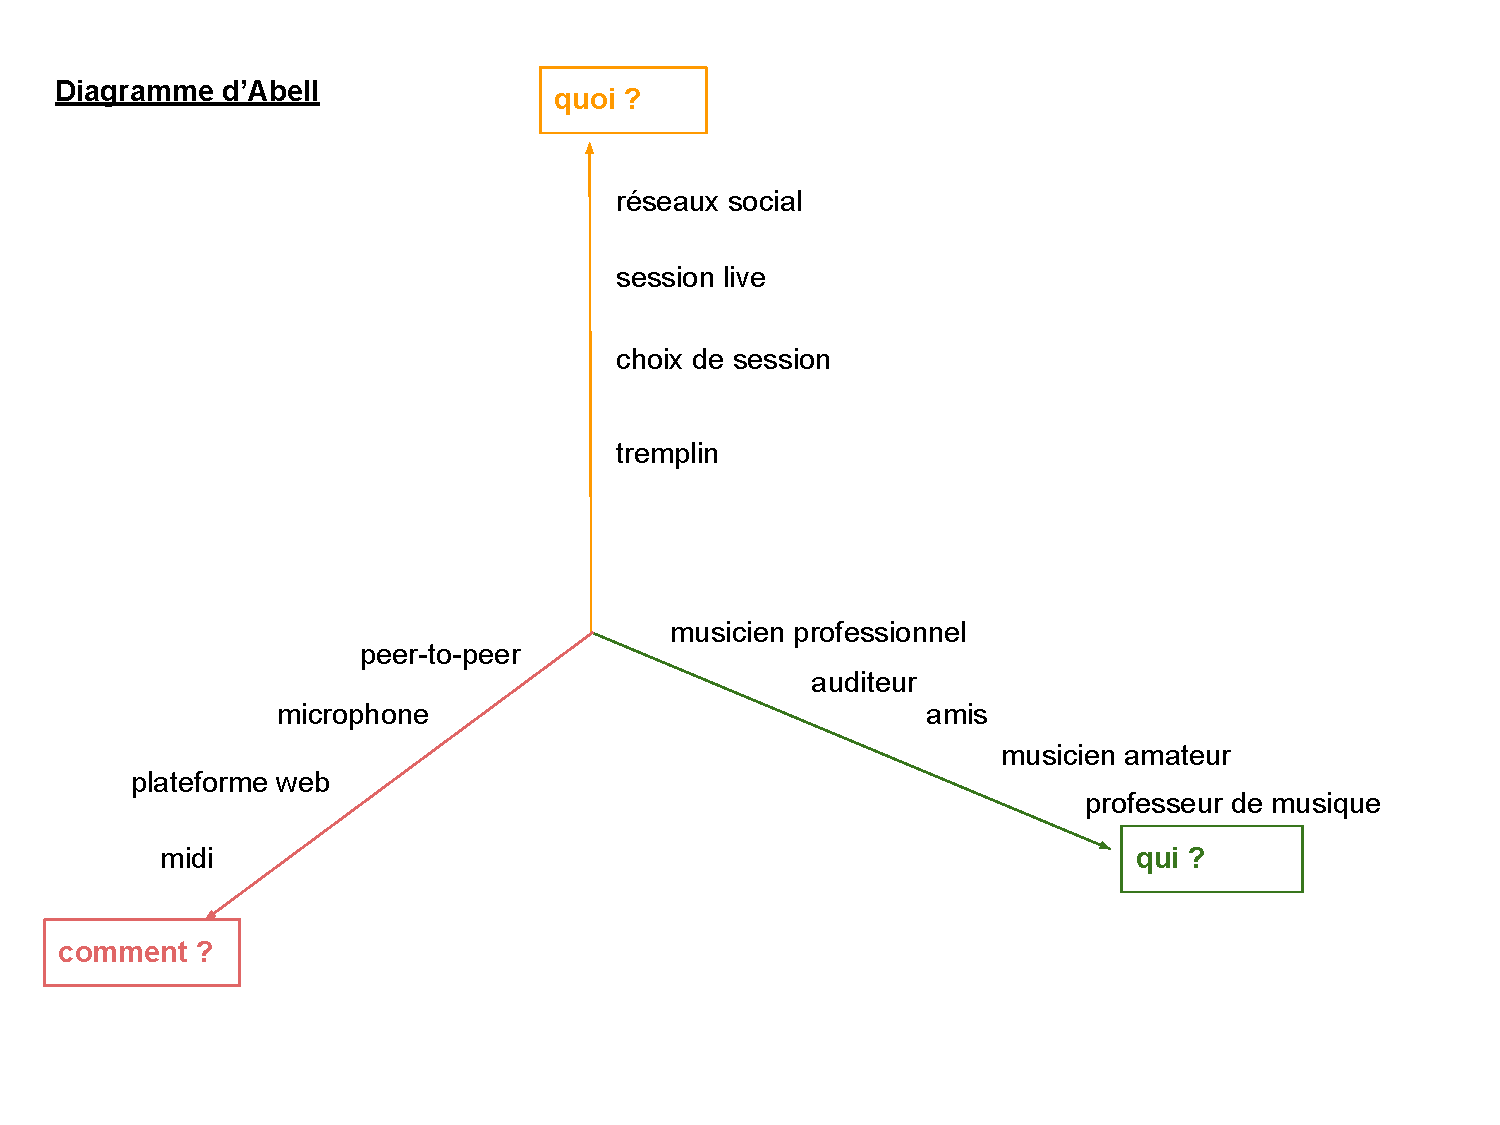
\includegraphics[width=400pt]{Abell.pdf}
    \caption{Diagramme d'Abell}
    \label{fig:diagrammeAbel}
\end{figure}

\begin{figure}[H]
    \centering
    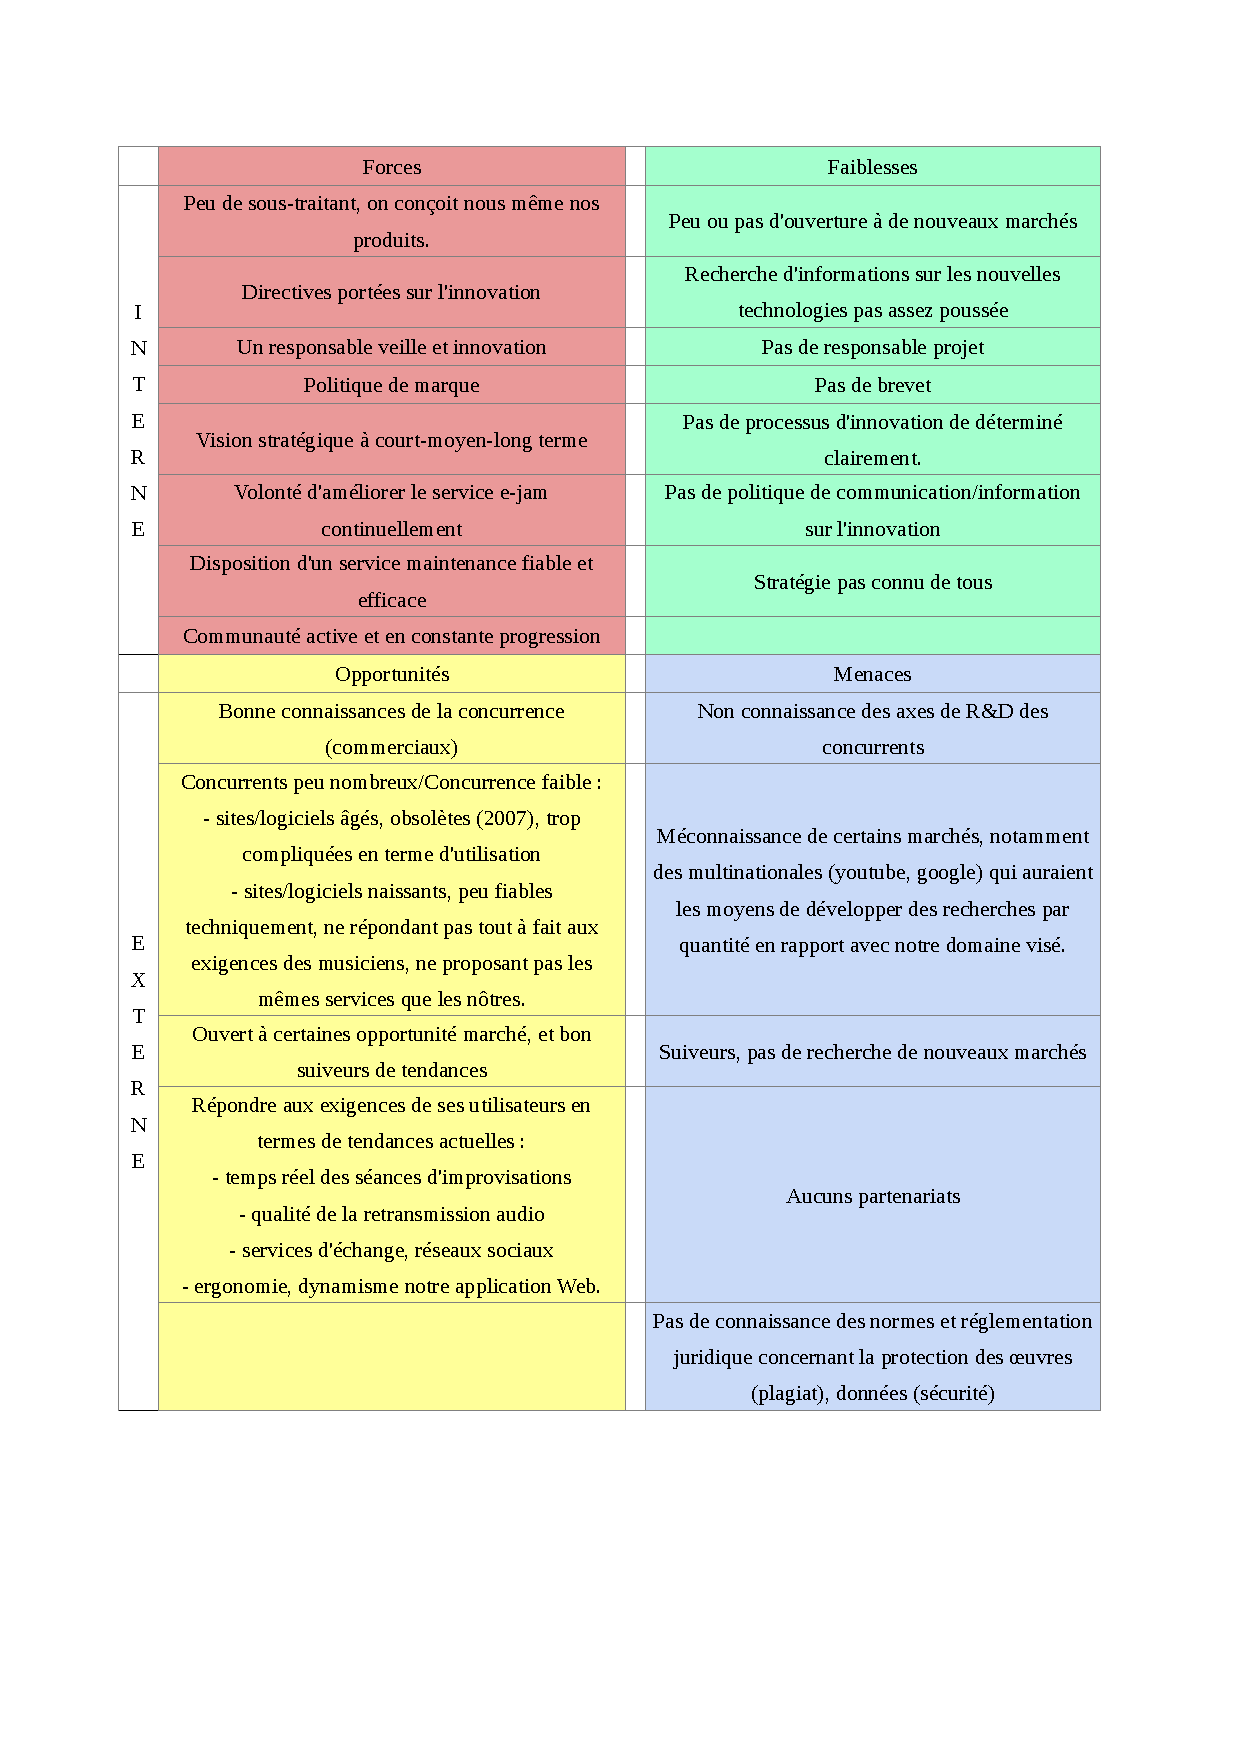
\includegraphics[scale=0.7]{SWOT.pdf}
    \caption{Matrice SWOT}
    \label{fig:SWOT}
\end{figure}

\end{document}
